%!TEX root = ../doc.tex
\pagenumbering{Roman}

\appendix
\chapter{Anhang}
\label{sec:Anhang}
Im Anhang dieses Dokumentes befinden sich nur die in der Arbeit referenzierten Codeausschnitte sowie die Aufgabenstellung. Alle in dieser Arbeit generierten Files sind auf dem ZHAW pool unter: \url{//shared.zhaw.ch/pools/t/T-IMS-SmartPro/Projekt/ROS-Industrial} zu finden.

\section{Offizielle Aufgabenstellung}
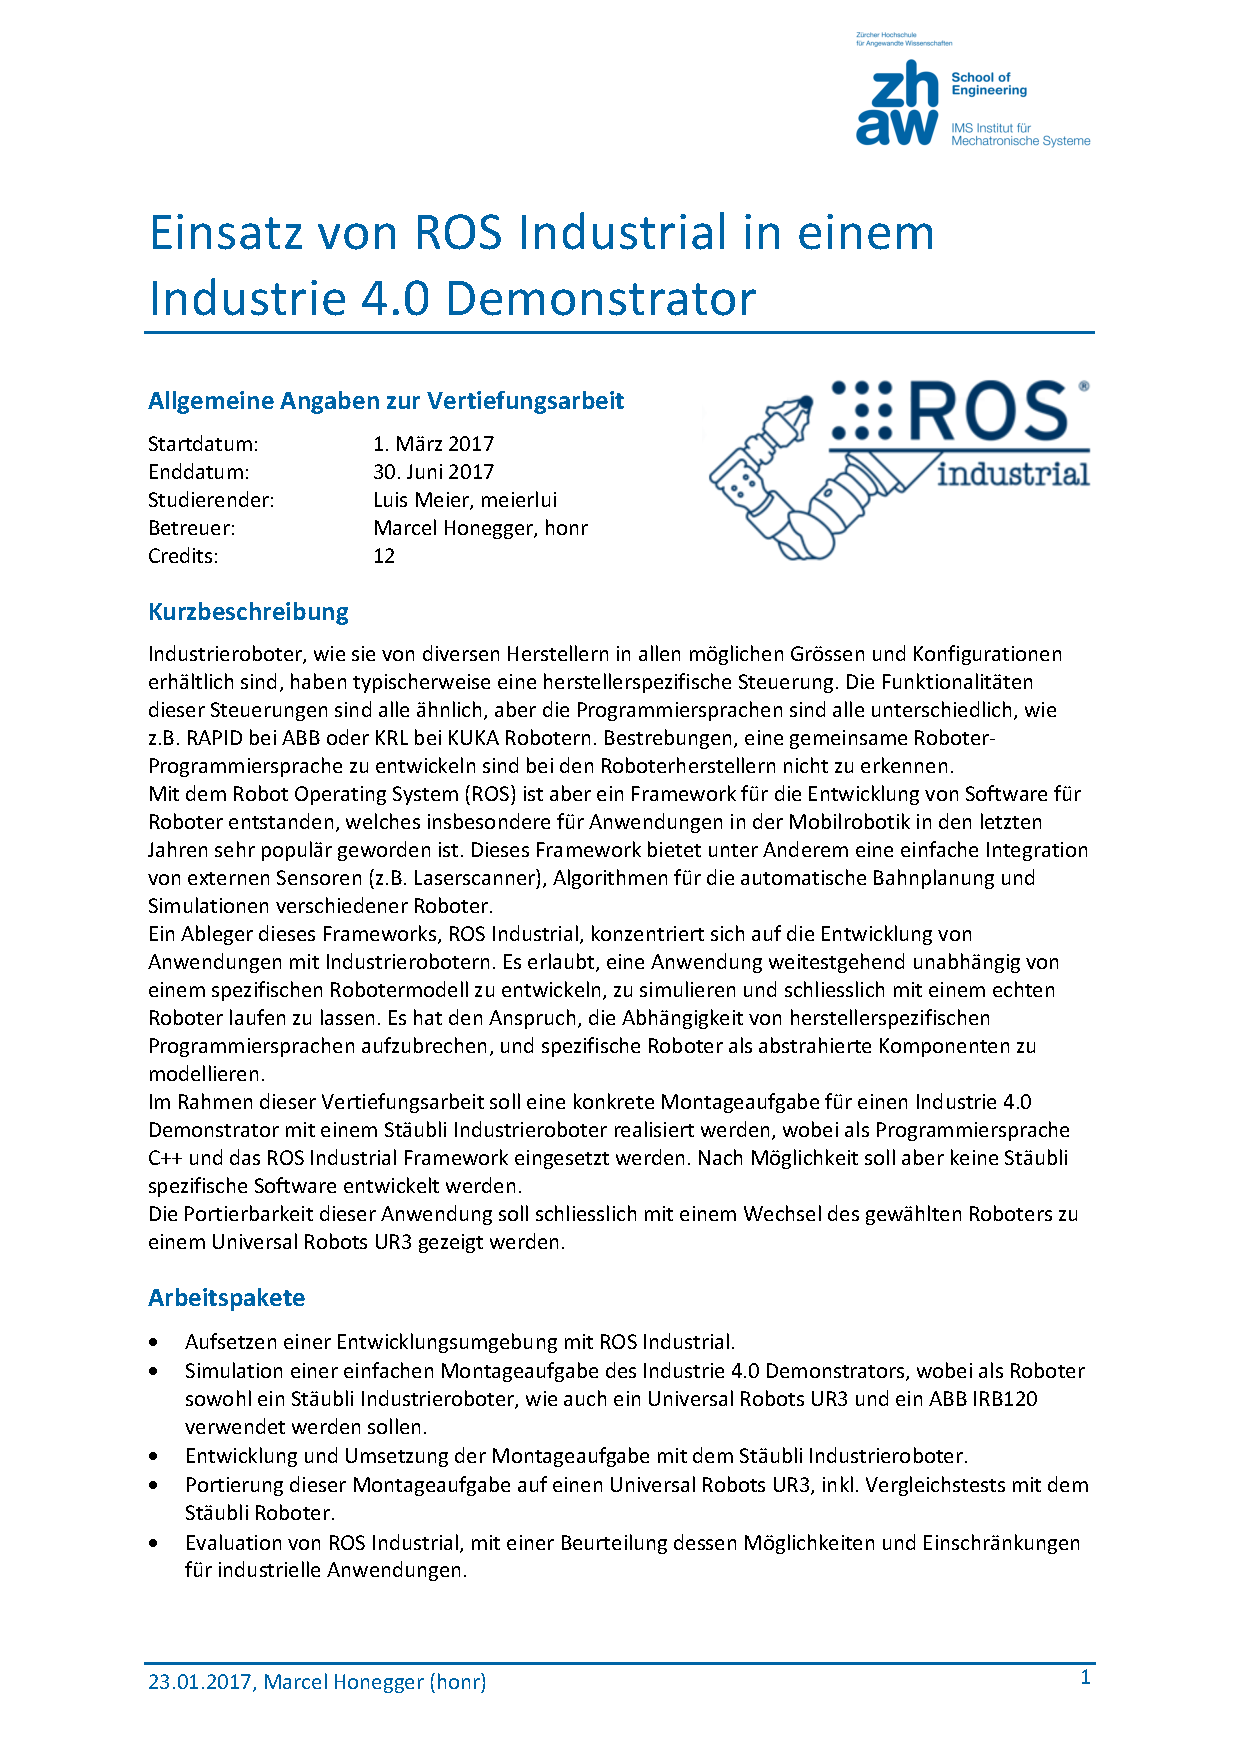
\includepdf{anhang/Aufgabenstellung.pdf}

\newpage
\section{Sourcecodefiles}
\subsection{Vollständige CMakeLists}\label{Anhang:Cmakelists}
\inputminted[bgcolor=white]{cmake}{anhang/CMakeLists.txt}

\newpage
\subsection{moveit\_planning\_execution.launch}\label{Anhang:MoveitVorlage}
\inputminted[bgcolor=white]{xml}{anhang/moveit_planning_execution.launch}

\newpage
\subsection{tx260l\_macro.xacro} \label{Anhang:Staublixacro}
\inputminted[bgcolor=white]{xml}{anhang/tx260l_macro.xacro}


